\documentclass{www2010-submission}

\usepackage{graphicx}
% \usepackage[left=2cm,top=1cm,right=3cm]{geometry}

\begin{document}
\setlength{\parindent}{0pt}
\setlength{\parskip}{.5ex plus 0.5ex minus 0.2ex}


% \setlength{\parskip}{8pt}
% \setlength{\parsep}{8pt}


\title{ drawnTogether -- a collaborative approach to virtual graffiti }

\author{ Jeremy Kelley, Kyumin Lee, \& Xiheng Zhang }

\date{\today}

\maketitle

\section{ User Study 1 }
\subsection{Interviewees}
We conducted nine people:

\begin{itemize}
\item (A) male, an iphone 3G S user
\item (B) male, a computer science graduate student
\item (C) female, a person who enjoys drawing
\item (D) male, an iPhone 3G S user
\item (E) male, a computer science graduate student
\item (F) male, a computer science graduate student
\item (G) male, professional graphic artist and iPhone 3G S user
\item (H) female, non-technical profession, non-iPhone user
\end{itemize}

\subsection{conducting user study}

Conducting the user study can involve multiple methods.  For our study, we took
an informal, guided conversational approach to gather the information.  We
provided a semi-structured questionnaire that our interviewers were to follow.

This questionnaire was divided up into multiple phases.

\subsubsection{ Introduction }

This phase consists of multiple steps:
\begin{itemize}
\item welcome and greetings
\item gather consent and completion of form
\item introduce the system in conversational form
\item communicate goals for this study
\end{itemize}

This phase is general housekeeping and provides for a welcoming and
customization period between the interviewer and interviewee.  Any general
questions are encouraged at this point about the general concept, but the
system has not been officially ``placed in their hands'' yet.

\subsection{ Facilitation }

In order gather information about usage, we will physically hand the users a
lo-fi representation of the drawnTogether interface in the form of a tangible,
translucent enclosure with cards that can swap out to represent the varying
views of the application.  When the user ``navigates'' between the views, the
interviewer will act as the computer and move the cards for the user.  The
benefits of this are numerous, but primarily, it allows us to iteratively
improve the interface and pilot new versions in a much faster way than
implementing the changes in software first.

We interviewed multiple individuals (eight total) over a period of three days.
The first six individuals used the same version of our interface.  The last two
used a modified version based on feedback gained from earlier interviews.  The
second version of our application views were very well received, as will be
seen in the following commentary.

For each interview, we began our questions with handing them the device, then
asking the following:
\begin{quote}
Is there anything particularly interesting about the concept of the
application?
\end{quote}

Most respondents actually felt the application to be quite interesting.
Respondent B, however, felt that it's merely a ``funny application'', and doubted if 
there would be enough situations for the system to be used.   He did provide
one possible  scenario. Imagine a group of architecture students
enter into one building to make a sketch of the inside structure of this
building. Each student can find whether the viewer around him or her has been
drawn or not. If not, he can add his sketch on the screen of the application.
If yes, he may ignore it and go to other places to draw or make some correction
based on others' drawings.  It was interesting to the researchers that even a
skeptic began to imagine practical, unforeseen collaborative uses.

Following the initial question, we followed with providing four erasable
markers of differing colors to the interviewee.  We had them ``navigate'' to
the drawing screen if he or she were on a different screen.  At this point, we
asked the following:

\begin{quote}
Can you draw a simple picture using multiple colors on the screen?
\end{quote}

With this question, we wanted to gauge the intuitiveness of the interface and
the user's ability to recognize visual affordances and their mapping to
intended tasks.  Person A asked ``Can I draw now?  What's the status of my
pen?''.  Several users touched the settings button before ever trying to draw,
with the purpose of exploring their options and tools before actually beginning
any sketch creation.  Person C immediately picked up a random pen (blue) and
began drawing on the screen.  When asked how they would change colors in the
application, the response was ``Oh\ldots  the settings page'', to which she
instantly and easily navigated to the page and chose the blue color.  Again,
with each navigation, the interviewer acted as the computer and moved the cards
as requested to transfer the user to different views.  Once in the setting
page, all users had an apparently clear understanding of how to manipulate the
current drawing color or erasure.

Multiple users asked about the tagging features visible on the settings page.
With minimal instruction from our facilitator, users understood the nature.
One thing was made clear to the developers with these questions, though.  The
ability to create tags and filter tags on the same view was a little confusing
and needs to be revisited.  The later revision used by the last two
interviewees provided a much clearer mapping and helped to eradicate most of
the confusion.

There were several questions about the appropriate time to tag a drawing or as
to the origin of the tags used for filtering.  These questions were quite
helpful in illuminating deficiencies with some of the feedback mechanisms
around the affordances related to tagging.

One interesting suggestion from multiple users was to add a voting feature for
a given location's sketches.  This way, a ranking per location could be used to
sort each location and be communicated on the map also.

Our next question was one which encouraged them to examine the map view, if
they had already not seen it:

\begin{quote}
Please navigate to the map view. {\it [pause for navigation]}
What pieces of information do you gather from this view?
\end{quote}

Once on the map, Person G mentioned ``Oh, I can see where other users sketches
are.  Cool''.  This was very satisfying to the researcher that the primary and
immediate purpose of the map was summed up so well.  User A asked, ``Can you 
show the sketches actual sketches from different locations on the map? In a
pop-up window?''


\subsection{Interview Completion}

In this phase, we attempted to provide a summary of each person's response and
to gather further clarification if needed.

We also ended with one final question, intended to spark a free form conversation:

\begin{quote}
Are there any recommendations you would make to improve your experience?
\end{quote}

Two individuals suggested moving the color palette from the setting page to the
bottom of the drawing view.  This would have the effect of drastically reducing
the interaction required for a meta task of changing the drawing color.  Several
users changed colors at least twice, so the benefits of this change seem
beneficial.  For the final two interviews, this change was adopted and proven
to be a valid enhancement immediately.  Person G used the modified drawing view
and changed colors five times while creating a sketch.  Person H changed colors
four times.  This was a definite, measurable improvement and allowed for a more
refined workflow for task completion.

The sacrifice of reduced drawing area was mitigated by removing the top bar
completely in the drawing view and adding navigational elements to the bottom
toolbar to allow for access to settings and the map.  This had no visible,
negative effect on the latter participants in the study on their ability to
navigate between views.  The changed views can be seen in Figure \ref{fig:chg}.

\begin{figure}
\centering
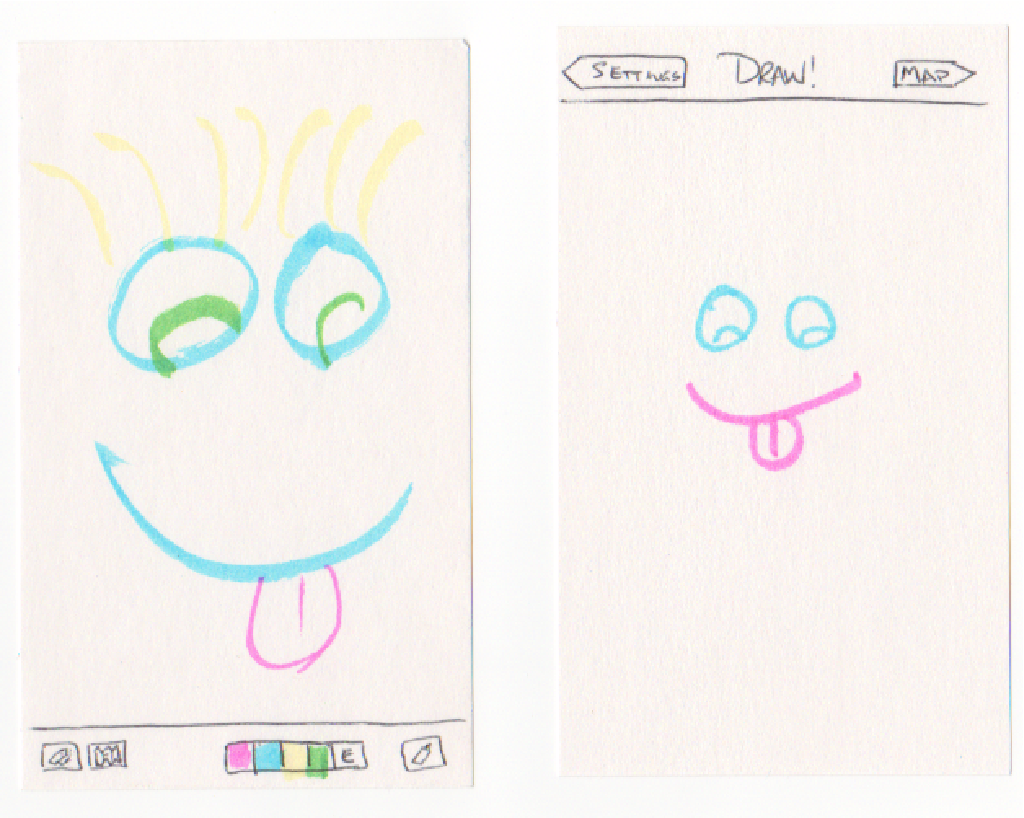
\includegraphics[width=.45\textwidth]{interface.pdf}
\caption{On the right, we see the modified drawing interface, with the color
pallete immediately visible at the bottom of the screen.  On the right, the
original interface requiring navigation away from the sketch to alter colors.}
\label{fig:chg}
\end{figure}

Another suggestion, offered by Person A, was to launch the application with the
map page initially.  Further conversation with the participant on this
consideration showed several potential benefits of adopting this.
\begin{itemize}
\item Participation feedback is immediately communicated by this macro approach
to making visible the locations containing sketches.  Each sketch becomes just
one minor data point on the geographical plot.
\item Users can immediately choose to change their location in order to either
add to an existing drawing or to create something new and unique
\item Community involvement is augmented by seeing participation.  If each map
pin is somehow annotated with the sketch age, a visual component could easily
communicate a temporal nature for each sketch showing which areas could benefit
from a ``fresh creation''.
\end{itemize}

In closing, almost all participants expressed an interest in getting this
application for their personal use.  


\end{document}
